cd ~/%!TEX root = ../dokumentation.tex


\chapter{Implementation}\label{cha:Implementation}

\section{Lexer}\label{sec:ImplementationLexer}

As mentioned in chapter \ref{sec:ConceptLexer} the implementation of the lexer consists of the definition of tokens in form of regular expression. The following paragraph presents defined tokens and their regular expressions.

\subsubsection{Ignored symbols}
It is possible to declare symbols that should be ignored. However, if a symbol is declared as ignored but is specially mentioned in another token, then if the sequence
of characters represent that token, the ignored symbol is not ignored. In this project, tabs and white spaces are ignored as they do not have any special meaning other than providing clarity.
Also, newlines are generally ignored because as can be seen in listing \ref{lst:Lexer_example_multiline} there are rules that cover multiple lines.

\begin{lstlisting}[basicstyle=\scriptsize	,caption= Multi line production rule,label= lst:Lexer_example_multiline]
<annotated_formula>    ::= <thf_annotated> | <tff_annotated> | <tcf_annotated> |
                           <fof_annotated> | <cnf_annotated> | <tpi_annotated>
\end{lstlisting}

Apart from the ignored symbols, there are 13 defined tokens:

\subsubsection{Expressions}

Expressions can either be of the type grammar, token, strict or macro. It is defined as a nonterminal symbol followed by the production symbol itself (::=,:==,:::,...). The nonterminal symbol and the production are merged to a single token and are not identified as two tokens to avoid ambiguity while parsing. If not it would be difficult for the parer to determine whether the nonterminal symbol that describes the rule is the start of a new rule or does still belong to the previous rule because as mentioned rules can cover multiple lines.

\textit{Regular expression of grammar expression:}  $'<\backslash w+>[\backslash s]*::='$

$\backslash w+$ matches any alphanumeric and underscore character that can occur more than one time.
$[\backslash s]*$ matches an arbitrary amount of white spaces.

\subsubsection{Nonterminal symbol}

A nonterminal symbol starts with \dq <\dq and ends with \dq >\dq. In between there is any arbitrary sequence of numbers, underscores and small or capital letters.

\subsubsection{Terminal symbol}

\subsubsection{Comment}

A comment is identified by the lexer as a start of a new line followed by a percentage sign followed by an arbitrary character and ends with a newline. Because the percentage sign is also part of the terminal symbols, it is necessary to check whether the percentage sign is in a newline because the terminal symbol is not because the percentage symbol when used as terminal symbol is embedded in square brackets.    

\subsubsection{Meta-Symbols}

Meta-Symbols include open and close parentheses \dq( )\dq, open and close square brackets \dq[ ]\dq, asterisks \dq *\dq and vertical bars \dq |\dq.

They are recognized by the symbol itself and have a greater meaning for the parser as they impact the to be build data structures. 

\subsubsection{Ambiguity}

The following example could either be matched as one comment token or as comment, grammar expression, non terminal symbol, terminal symbol, non terminal symbol.
This ambiguity is solved because by convention the lexer matches the longest possible token, the sequence of characters is matched as one comment.
\begin{lstlisting}[basicstyle=\scriptsize	,caption= Commented out production rule,label= lst:Lexer_example]
%----   <formula_role> ::= <user_role>-<source>
\end{lstlisting}
\section{Parser}\label{sec:ImplementationParser}

The parser is taking the tokens from the lexer and matches them to defined production rules.




comment block reimplement equal operator

\subsection{Data types}\label{sec:ImplementationDataTypes}
Figure \ref{fig:ImplementationUMLExpressions} contains the UML modelling of the data types described in section \ref{sec:ConceptParserDataStructure}.
\begin{figure}[H]
\centering
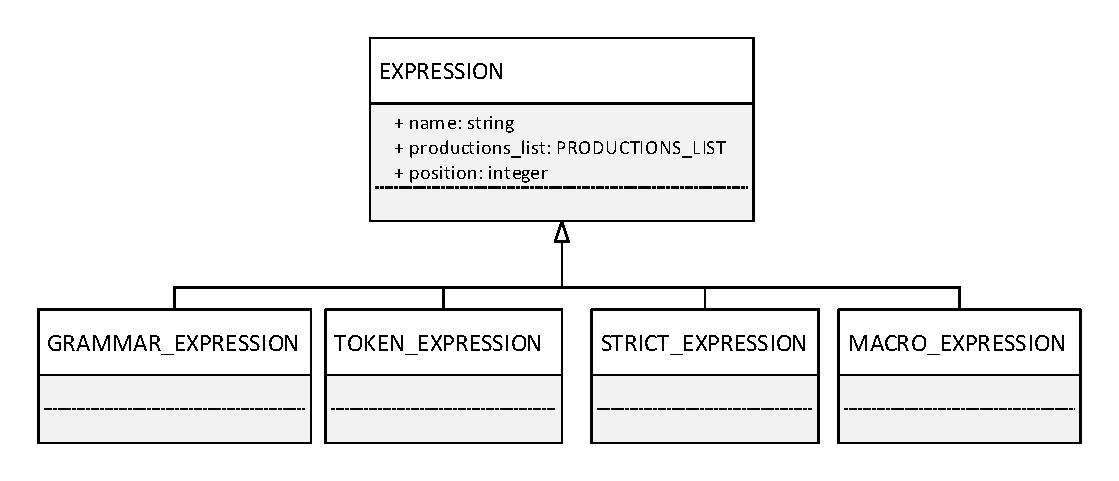
\includegraphics[width=1\textwidth]{images/uml_data_types_expressions.pdf}
\caption{UML diagram for expressions}
\label{fig:ImplementationUMLExpressions}
\end{figure}


\begin{figure}[H]
\centering
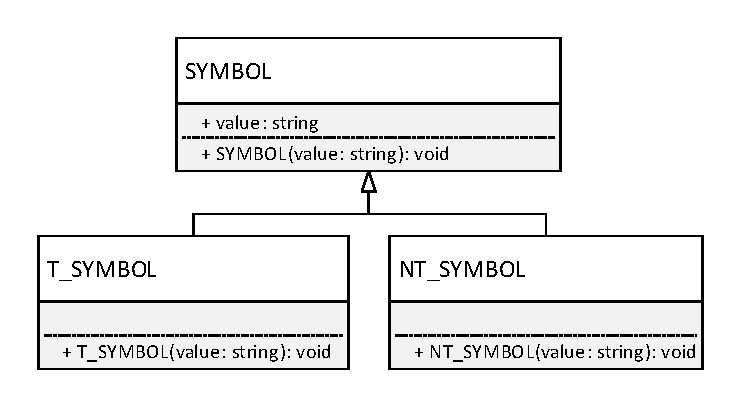
\includegraphics[width=.7\textwidth]{images/Implementation_parser_symbol_uml.pdf}
\caption{Symbols UML diagram}
\label{fig:ImplementationUMLSymbols}
\end{figure}


\subsection{Defined grammar}\label{sec:ImplementationGrammar}

- Input of parser is formal grammar \\

The grammar is formally specified $G = (N,\sum,P,S)$.

$N$ is the set of nonterminal symbols. The set includes grammar list, comment block, grammar expression, token expression, strict expression, macro expression, productions list, production, xor productions list, t symbol production and production element.

$\sum$ is the set of terminal symbols. Terminal symbols of the specified grammar are the tokens generated by the lexer (see \ref{sec:ConceptLexer}).

$P$ is the set of production rules that are presented in the following. 

A grammar list implies a comment block, the four expressions or a grammar list followed by the expressions.

\begin{align*}
	grammar\;list\; \rightarrow\; &comment\;block
	     		\mid grammar\;expression  \\
			   &\mid token\;expression
                \mid strict\;expression\\
               &\mid macro\;expression \\
               &\mid grammar\;list\;\;\;grammar\;expression\\
               &\mid grammar\;list\;\;\;strict\;expression \\
               &\mid grammar\;list\;\;\;macro\;expression \\
               &\mid grammar\;list\;\;\;comment\;block               
\end{align*}

A comment block is either a comment or a comment block with a comment.

\begin{align*}
    comment\;block\; \rightarrow\; &\textbf{comment}
                \mid comment\;block\;\;\textbf{comment}
\end{align*}

The four expressions are the expression token followed by their productions list. Grammar expression has a special case without a productions list because the production rule $ <null> ::= $ has nothing on the right side. 

\begin{align*}
	grammar\;expression\; \rightarrow\; &\textbf{l grammar expression}\;\;productions\;list \\ 
               &\mid \textbf{l grammar expression} 
\end{align*}
\begin{align*}        
	token\;expression\; \rightarrow\; &\textbf{l token expression} \;\;productions\;list \\ \\
	strict\;expression\; \rightarrow\; &\textbf{l strict expression} \;\;productions\;list \\ \\
	macro\;expression\; \rightarrow\; &\textbf{l macro expression} \;\;productions\;list 
\end{align*}

Productions list and xor productions list imply either a production or a productions list alternative symbol production.

\begin{align*}
	productions\;list\; \rightarrow\; &production \\
               &\mid productions\;list\;\;\textbf{alternative symbol} \;production \\ \\                   
	xor\;productions\;list\; \rightarrow\; &production \\
               &\mid xor\;productions\;list\;\;\textbf{alternative symbol}\;production 
\end{align*}

T symbol production is either a t symbol or a t symbol/repetition symbol/ alternative symbol embedded in square brackets.

\begin{align*}
	t\;symbol\;production\; \rightarrow\; & \textbf{open square bracket \; t symbol} \\ &\textbf{close square bracket}\\
               &\mid \textbf{open square bracket \; repetition symbol} \\ &\textbf{close square bracket}\\
               &\mid \textbf{open square bracket \; alternative symbol } \\ &\textbf{close square bracket}\\
               &\mid \textbf{t symbol} 
\end{align*}

Production element can be replaced by a nt symbol or by a nt symbol in square brackets or nt symbol repetition. In the case of repetition or square brackets the production element is categorized as optional when in square brackets or as repetition when followed by the repetition symbol. The same applies to t symbol production. A production element can also only be square brackets only.

 

\begin{align*}
	production\;element\; \rightarrow\; & \textbf{open square bracket \; nt symbol} \\ 
			   &\textbf{close square bracket}\\
               &\mid \textbf{nt symbol \; repetition symbol} \\
               &\mid t\;symbol\;production\;\; \textbf{repetition symbol} \\
               &\mid \textbf{open square bracket \; close square bracket} \\
               &\mid \textbf{nt symbol} \\
               &\mid t\; symbol\; production 
\end{align*}




\begin{align*}
	production\; \rightarrow\; &production\; element
                \mid production\;\; production\; element \\
               &\mid \textbf{open parenthesis}\;\; xor\; \;productions\; list\;\; \\
               &\textbf{close parenthesis} \\
               &\mid \textbf{open parenthesis}\;\; production\;\; \textbf{close parenthesis} \\
               &\mid production \;\;\textbf{open parenthesis}\;\; production \\
               &\textbf{close parenthesis} \\
               &\mid production\;\; \textbf{open parenthesis} \;\;xor \;productions\; list\\
               &\textbf{close parenthesis} \\
               &\mid \textbf{open parenthesis} \;\;production \;\;\textbf{close parenthesis} \\
               &production \\
               &\mid \textbf{open parenthesis}\;\; xor\; productions\; list\\ 
               &\textbf{close parenthesis}\;\; production \\
               &\mid \textbf{open parenthesis}\;\; production\;\; \textbf{close parenthesis} \\
               &\textbf{repetition symbol}\\
               &\mid production\;\; \textbf{open parenthesis} \;\;production \\
               &\textbf{close parenthesis \; repetition symbol}
\end{align*}


- $S$: grammar list, start symbol is not mentioned, per convention by \ac{PLY} first rule found (top level rule)

Listing \ref{lst:Parser_example_productionelement} shows the production rule of the nonterminal $<tfx tuple>$ as well as the tokens that have been generated by the lexer.

\begin{lstlisting}[basicstyle=\scriptsize	,caption= Production element,label= lst:Parser_example_productionelement]
<tfx_tuple>            ::= [] | [<tff_arguments>]
is made of tokens:
l grammar expression open square bracket close square bracket alternative symbol open square bracket nt symbol close square bracket
\end{lstlisting}

The resulting parse tree can be seen in figure \ref{fig:ImplementationParsing}. 

\begin{figure}[H]
\begin{tikzpicture}[
  ->,>=stealth',
  level/.style={level distance=1.5cm,sibling distance=4cm},
  level 2/.style={sibling distance=6cm},
  level 3/.style={sibling distance=5cm},
  level 5/.style={level distance=2cm, sibling distance=4cm},
  level 6/.style={level distance=2cm, sibling distance=4cm}
]
\node {grammar list}
    child{ node  {grammar expression} 
    		child{ node {\textbf{l grammar expression}}}
            child{ node {productions list} 
                child{ node  {productions list}
                	child {node {production}
                		child {node {productions element}
                			child{node {\textbf{\shortstack{open square bracket \\ close square bracket}}}}}}} 
                child{ node  {\textbf{alternative symbol}}}
                child{ node  {production}
                	child {node {productions element}
                		child{node {\textbf{\shortstack{open square bracket \\ nt symbol \\ close square bracket }}}}}}
                				}}
   
; 
\end{tikzpicture}
\caption{Parsing example}
\label{fig:ImplementationParsing}
\end{figure}
                
                
                
\section{Graph generation}\label{sec:ImplementationGraphGeneration}

To generate the graph of a given grammar three algorithms are needed that will be explained in the following. 

The algorithm $buildGraphRek$ calls the function $searchProductionsListForNT$ that appends children of a node to the nodes list of children. The algorithm is first called with the start symbol. 
After the children of a node have been appended to the node, every child calls the algorithm resulting in appending their own children to their children's list. 

\begin{algorithm}[H]
\caption{Graph Generation Algorithm: buildGraphRek}
\begin{algorithmic}[1] 
\Require node
%\ENSURE $y = x^n$
\State searchProductionsListForNT(node, node.productionsList)
\If {node has children}
	\ForAll {children}
		\State buildGraphRek(child)
	\EndFor
\EndIf
\end{algorithmic}
\end{algorithm}

The right side of a production rule is stored in a productions list. For identifying the nonterminal or terminal symbols in the productions lists, a loop iterates through all elements of the productions list. Each element is a production and calls the function $searchProductionForNT$. This function identifies the children of the given element who are then appended to the node.

\begin{algorithm}[H]
\caption{Algorithm for extracting productions from productions list: searchProductionsListForNT}
\begin{algorithmic}[1] 
\Require node, productionsList
\ForAll {elements in productionsList}
	\State children = new empty list
	\State searchProductionForNT(node, element in productionsList, children)
	\State append children to node
\EndFor
\end{algorithmic}
\end{algorithm}

The goal is to identify the nonterminal symbols. Therefore it is checked if the production is a nested production and if so, the same function is called again. If the production is a XOR production list the function $searchProductionsListForNT$ is called to break down the productions list. If the production element is a nonterminal symbol the element is searched in the node dictionary to get the node where the element is on the left side. This element is then appended to a list of children. It is possible that an element appears multiple times on the left side if it is presented by multiple expressions. In this case each element is appended to the list of children.

\begin{algorithm}[H]
\caption{Algorithm for appending children to node: searchProductionForNT}
\begin{algorithmic}[1] 
\Require node, productionsElement, children
\ForAll {elements in productionsElementList}
	\If {element is  a production}
		\State {searchProductionForNT(node, element, children)}
	\ElsIf {element is a XOR productions list}
		\State {searchProductionsListForNT}
	\ElsIf {element is a nonterminal symbol}
		\State find element(s) in node dictionary
		\State append element(s) to children
	\EndIf
\EndFor
\end{algorithmic}
\end{algorithm}

\subsection{Removing of blocked productions}
The productions that should be blocked are specified in the control file.  
Algorithm \ref{sec:remove_blocked_productions}
\begin{algorithm}[H]
\caption{Removing blocked productions}
\begin{algorithmic}[1] 
\Require control\textunderscore string
\State lines = control\textunderscore string.splitlines()
\State start\textunderscore symbol = lines[0]
\State delete lines[0]
\ForAll {line in lines}
	\State data = line.splitBy(",")
	\State nonterminal\textunderscore name = data[0]
	\State rule\textunderscore symbol = data[1]
	\State rule\textunderscore type = determineRuleType(rule\textunderscore symbol)
	\State delete data[0:2]
	\State data = parseInteger(data)
	\State data.sortReverse()
	\ForAll {index in data}
		\State node = this.nodes\textunderscore dictionary.get(Node(nonterminal\textunderscore name, rule\textunderscore type))
		\State delete node.productions\textunderscore list.list[index]
		\State delete node.children[index]
	\EndFor
\EndFor
\end{algorithmic}
\label{alg:remove_blocked_productions}
\end{algorithm}

\subsection{Determination of the remaining reachable productions}
\subsubsection{Removing non-terminating symbols}
\begin{algorithm}[H]
\caption{Removing blocked productions}
\begin{algorithmic}[1] 
\Require start\textunderscore node
\State terminating = new set()
\State temp\textunderscore terminating = new set()
\While {True}
	\State visited = new set()
	\State this.find\textunderscore non\textunderscore terminating\textunderscore symbols(start\textunderscore node, temp\textunderscore terminating, visited)
	\If {terminating == temp\textunderscore terminating}
		\State break
	\Else
		\State terminating = temp\textunderscore terminating
	\EndIf
\EndWhile
\State delete\textunderscore non\textunderscore terminating\textunderscore productions\textunderscore (start\textunderscore node, terminating, visited)
\State delete\textunderscore non\textunderscore terminating\textunderscore nodes(terminating)
\end{algorithmic}
\label{alg:remove_non_terminating_symbols}
\end{algorithm}


\section{GUI}\label{sec:ImplementationGUI}
Tkinter and PyQt have been evaluated as a basis for the GUI.
-pyqt offers checkboxes in treeviews
\begin{figure}[H]
\centering
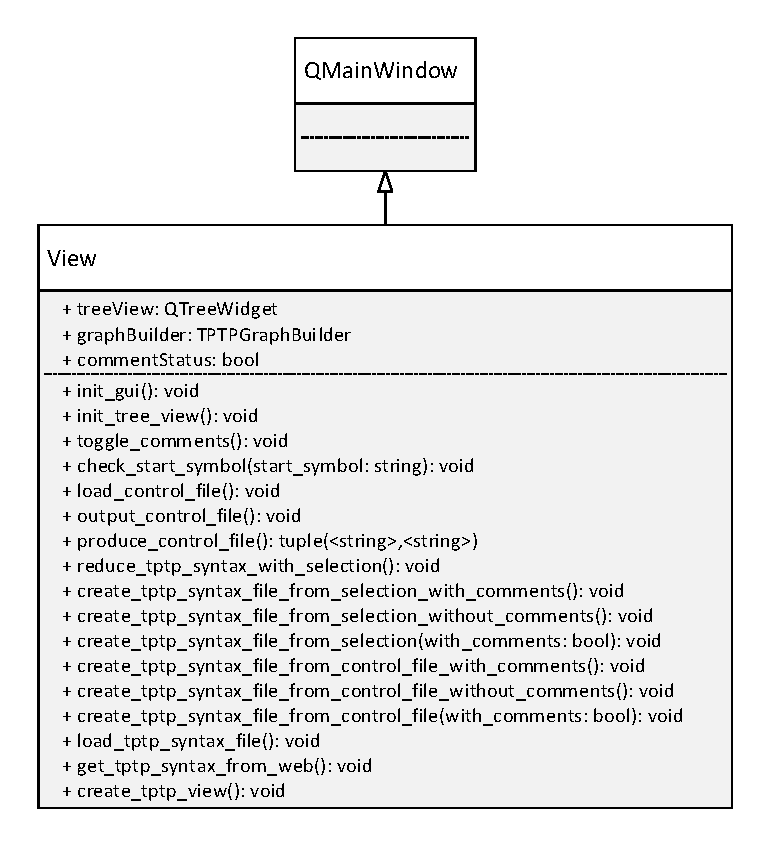
\includegraphics[width=0.6\textwidth]{images/Implementation_view_class_diagramm.pdf}
\caption{View UML class diagram}
\label{fig:ImplementationViewClassDiagram}
\end{figure}
-todo uml diagram View
\subsection{Display rules}\label{sec:ImplementationGUIDisplayRules}

\subsection{Toggle comments}\label{sec:ImplementationGUIToggleComments}
\subsection{Import control file}\label{sec:ImplementationGUIImportControlFile}
\subsection{Import \ac{TPTP} syntax from the internet}\label{sec:GUI}
\section{Command-line interface}\label{sec:ImplementationCommandLineInterface}
For the command-line interface (see section \ref{sec:ConceptCommandLineInterface}) the python module argparse is used.
todo more, explain and explain why

Table \ref{tbl:ImplementationCommandLineParameters} provides an overview about the needed command-line arguments.
The syntax file location and the control file location has to be specified.
Specifying an output path and file name is optional, by default the output filename will be \textit{output.txt}.\\
Additionally, the help description can be opend by using the \textit{-h} option
\begin{table}[H]
\centering
\caption{Command-line interface parameters}
\begin{adjustbox}{width=1\textwidth, center=\textwidth}
\renewcommand{\arraystretch}{2}
\begin{tabular}{llll}
\textbf{Name} & \textbf{Short form} & \textbf{Default} & \textbf{Description}\\\hline
-{}-grammar & -g & None & \ac{TPTP} syntax file path and filename\\
-{}-control & -c & None &  Control file path and filename\\
-{}-output & -o & output.txt & Output file path and filename (optional)
\end{tabular}
\end{adjustbox}
\label{tbl:ImplementationCommandLineParameters}
\end{table}

With the argparse module a command-line parser object can be created and parameters can be added to that object.
In the first line of \ref{lst:ImplementationArgparseParserConfiguration} the command-line parser object is created with a description.
Lines two to four contatin the specification of the accepted arguments.
In addition to the name and short form of the name, the type, a help message, and wether the parameter is optional or not can be specified.
Default values for arguments can also be specified.
If no default value is specified and if the argument is not passed it will have the value \textit{None}.
Argparse automatically checks the given conditions, for example if a required argument is not given and displays an error message if that is the case.
\begin{lstlisting}[language=Python, basicstyle=\scriptsize	,caption= Argparse command-line parser configuration,label= lst:ImplementationArgparseParserConfiguration]
self.argument_parser = argparse.ArgumentParser(description='Extract sub-syntax using TPTP syntax file and a control file')
self.argument_parser.add_argument('-g', '--grammar', metavar='', type=str, required=True, help='path of the TPTP syntax file')
self.argument_parser.add_argument('-c', '--control', metavar='', type=str, required=True, help='path of the control file')
self.argument_parser.add_argument('-o', '--output', metavar='', type=str, required=False, help='optional output file name (default output.txt)', default= "output.txt")
\end{lstlisting}

Argparse will also automatically create the help output by using the descriptions provided when configuring the argument parser.


-argparse Python offers a library for command-line interfaces.
-options for path to grammar and control file
-option for output path

-todo describe seperation of gui and why
